\chapter{The Four Major Problems}
\begin{flushleft}
    Monopoly, centralization of computing power, high energy consumption, and the incompleteness of existing PoCs have become the four major problems in the Crypto industry. From the beginning of its design, BHD is aimed at solving the four major problems.
\end{flushleft}
\section{Monopoly}
\begin{flushleft}
    Since its inception, Bitcoin has always had the mission to solve financial institutions’ crisis of confidence and issue of monopoly. Since the financial crisis in 2008, Nakamoto believed that the centralization of the financial system would lead to repetition of the history, thus decentralization could be an effective solution for the economy.
\end{flushleft}
\begin{flushleft}
    \centering\textbf{The greatest financial crises in the past 90 years}
\end{flushleft}
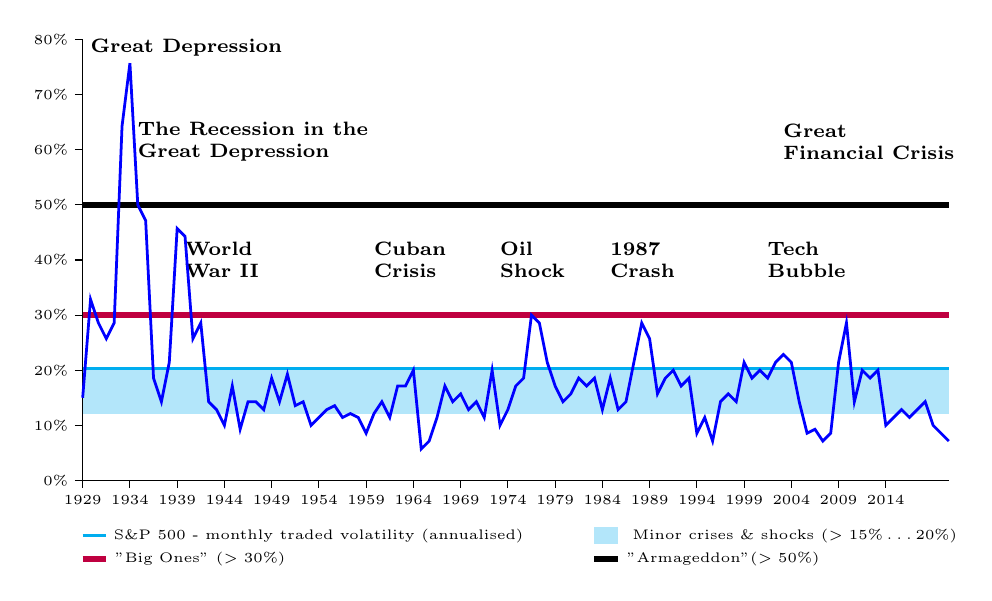
\begin{tikzpicture}
    \scriptsize
    \draw (0,5.5) node[align=left,right]{\textbf{Great Depression}};
    \draw (0.6,4.3) node[align=left,right]{\textbf{The Recession in the}\\\textbf{Great Depression}};
    \draw (8.8,4.3) node[align=left,right]{\textbf{Great}\\\textbf{Financial Crisis}};
    \draw (1.2,2.8) node[align=left,right]{\textbf{World}\\\textbf{War II}};
    \draw (3.6,2.8) node[align=left,right]{\textbf{Cuban}\\\textbf{Crisis}};
    \draw (5.2,2.8) node[align=left,right]{\textbf{Oil}\\\textbf{Shock}};
    \draw (6.6,2.8) node[align=left,right]{\textbf{1987}\\\textbf{Crash}};
    \draw (8.6,2.8) node[align=left,right]{\textbf{Tech}\\\textbf{Bubble}};
    \tiny
    \draw (0,0) -- (11,0);
    \draw (0,0) -- (0,5.6);
    \draw (0,0.1) -- (0,-0.1) node[align=left,below]{1929};
    \draw (0.6,0) -- (0.6,-0.1) node[align=left,below]{1934};
    \draw (1.2,0) -- (1.2,-0.1) node[align=left,below]{1939};
    \draw (1.8,0) -- (1.8,-0.1) node[align=left,below]{1944};
    \draw (2.4,0) -- (2.4,-0.1) node[align=left,below]{1949};
    \draw (3.0,0) -- (3.0,-0.1) node[align=left,below]{1954};
    \draw (3.6,0) -- (3.6,-0.1) node[align=left,below]{1959};
    \draw (4.2,0) -- (4.2,-0.1) node[align=left,below]{1964};
    \draw (4.8,0) -- (4.8,-0.1) node[align=left,below]{1969};
    \draw (5.4,0) -- (5.4,-0.1) node[align=left,below]{1974};
    \draw (6.0,0) -- (6.0,-0.1) node[align=left,below]{1979};
    \draw (6.6,0) -- (6.6,-0.1) node[align=left,below]{1984};
    \draw (7.2,0) -- (7.2,-0.1) node[align=left,below]{1989};
    \draw (7.8,0) -- (7.8,-0.1) node[align=left,below]{1994};
    \draw (8.4,0) -- (8.4,-0.1) node[align=left,below]{1999};
    \draw (9.0,0) -- (9.0,-0.1) node[align=left,below]{2004};
    \draw (9.6,0) -- (9.6,-0.1) node[align=left,below]{2009};
    \draw (10.2,0) -- (10.2,-0.1) node[align=left,below]{2014};
    \draw (-0.1,0) node[align=left,left]{$0\%$} -- (0,0);
    \draw (-0.1,0.7) node[align=left,left]{$10\%$} -- (0,0.7);
    \draw (-0.1,1.4) node[align=left,left]{$20\%$} -- (0,1.4);
    \draw (-0.1,2.1) node[align=left,left]{$30\%$} -- (0,2.1);
    \draw (-0.1,2.8) node[align=left,left]{$40\%$} -- (0,2.8);
    \draw (-0.1,3.5) node[align=left,left]{$50\%$} -- (0,3.5);
    \draw (-0.1,4.2) node[align=left,left]{$60\%$} -- (0,4.2);
    \draw (-0.1,4.9) node[align=left,left]{$70\%$} -- (0,4.9);
    \draw (-0.1,5.6) node[align=left,left]{$80\%$} -- (0,5.6);
    \draw[line width=2pt] (0,3.5) -- (11,3.5);
    \draw[purple,line width=2pt] (0,2.1) -- (11,2.1);
    \draw[cyan,line width=2pt] (0,1.4) -- (11,1.4);
    \fill[cyan!30] (0,1.4) rectangle (11,0.85);
    \draw[blue,line width=1pt] (0,1.05) -- (0.1,2.3) -- (0.2,2.0) -- (0.3,1.8) -- (0.4,2) -- (0.5,4.5) -- (0.6,5.3) -- (0.7,3.5) -- (0.8,3.3) -- (0.9,1.3) -- (1,1) -- (1.1,1.5) -- (1.2,3.2) -- (1.3,3.1) -- (1.4,1.8) -- (1.5,2) -- (1.6,1) -- (1.7,0.9) -- (1.8,0.7) -- (1.9,1.2) -- (2,0.65) -- (2.1,1) -- (2.2,1) -- (2.3,0.9) -- (2.4,1.3) -- (2.5,1) -- (2.6,1.35) -- (2.7,0.95) -- (2.8,1) -- (2.9,0.7) -- (3,0.8) -- (3.1,0.9) -- (3.2,0.95) -- (3.3,0.8) -- (3.4,0.85) -- (3.5,0.8) -- (3.6,0.6) -- (3.7,0.85) -- (3.8,1) -- (3.9,0.8) -- (4,1.2) -- (4.1,1.2) -- (4.2,1.4) -- (4.3,0.4) -- (4.4,0.5) -- (4.5,0.8) -- (4.6,1.2) -- (4.7,1) -- (4.8,1.1) -- (4.9,0.9) -- (5,1) -- (5.1,0.8) -- (5.2,1.4) -- (5.3,0.7) -- (5.4,0.9) -- (5.5,1.2) -- (5.6,1.3) -- (5.7,2.1) -- (5.8,2) -- (5.9,1.5) -- (6,1.2) -- (6.1,1) -- (6.2,1.1) -- (6.3,1.3) -- (6.4,1.2) -- (6.5,1.3) -- (6.6,0.9) -- (6.7,1.3) -- (6.8,0.9) -- (6.9,1) -- (7,1.5) -- (7.1,2) -- (7.2,1.8) -- (7.3,1.1) -- (7.4,1.3) -- (7.5,1.4) -- (7.6,1.2) -- (7.7,1.3) -- (7.8,0.6) -- (7.9,0.8) -- (8,0.5) -- (8.1,1) -- (8.2,1.1) -- (8.3,1) -- (8.4,1.5) -- (8.5,1.3) -- (8.6,1.4) -- (8.7,1.3) -- (8.8,1.5) -- (8.9,1.6) -- (9,1.5) -- (9.1,1) -- (9.2,0.6) -- (9.3,0.65) -- (9.4,0.5) -- (9.5,0.6) -- (9.6,1.5) -- (9.7,2) -- (9.8,1.0) -- (9.9,1.4) -- (10,1.3) -- (10.1,1.4) -- (10.2,0.7) -- (10.3,0.8) -- (10.4,0.9) -- (10.5,0.8) -- (10.6,0.9) -- (10.7,1) -- (10.8,0.7) -- (10.9,0.6) -- (11,0.5);
    \draw[cyan,line width=1pt] (0,-0.7) -- (0.3,-0.7) node[align=left,right,black]{S$\&$P 500 - monthly traded volatility (annualised)};
    \draw[cyan!30,line width=6pt] (6.5,-0.7) -- (6.8,-0.7) node[align=left,right,black]{Minor crises $\&$ shocks ($> 15\% \dots 20\%$)};
    \draw[purple,line width=2pt] (0,-1) -- (0.3,-1) node[align=left,right,black]{"Big Ones" ($> 30\%$)};
    \draw[line width=2pt] (6.5,-1) -- (6.8,-1) node[align=left,right,black]{"Armageddon"($> 50\%$)};
\end{tikzpicture}
\begin{flushleft}
    So after all these years, what is the current status of Bitcoin?
\end{flushleft}
\begin{flushleft}
    The figure below shows value curve of the entire cryptocurrency market led by Bitcoin. Does it not look like fluctuations in the financial crisis cycle? Which brings us to think if Bitcoin is still decentralized.
\end{flushleft}
\begin{flushleft}
    The technology of Bitcoin-core is controlled by the core developers, and the code update speed is very slow, which can be described as code-centralization. Bitcoin's computing power is tremendous, ordinary people and personal computers cannot take part and can only trade in exchanges, which indicates hash-power-centralization. Bitcoin's block generation time is relatively slow, about 10 minutes per block, single digit TPS (Transaction per second) cannot provide the same experience as the current internet. Bitcoin core wallet did not make any UI/UX enhancement in ten years, and there is neither a core mobile version, nor any consideration of the current user experience, which indicates user-experience-centralization. Some people are planning to deploy lightning network, allowing more centralized companies to join the nodes, turning the Bitcoin system into a centralized payment system with far worse user experience than visa.
\end{flushleft}
\begin{flushleft}
    Many believes that the existing Bitcoin system needs to be changed or overturned, keeping the decentralization spirit and involve everyone in this revolution. BHD has a more economical decentralization approach, using lower cost storage instead of CPU/GPU power. If we believe that centralization can cause crisis to reappear, then we need to know that monopoly has to be eliminated to avoid any risk of potential crisis in the crypto world.
\end{flushleft}
\section{Power Centralization}
\begin{flushleft}
    We mentioned, the main reason for Bitcoin to prevail and be successfully used as the digital money is that its hash power has been maintained at a relatively high level. In 2017, Bitcoin hash power was 4400P, daily production was 1,800 coins, every peta hash power generated 0.4 Bitcoin on average, and consisted of 166 units of 6 tera hash power mining machine. Here comes the issue, the price of Bitcoin can be influenced by mining machine manufacturers through adjusting the price of the mining machine. Thus as crypto currency participants anticipate an increase in Bitcoin's earnings, everyone is willing to mine with higher hash power machines, and enjoy a higher possibility to get rewards through packaging. The top four companies in Bitcoin mining account for about $53\%$ of the mining share; The Ethereum system has a higher concentration ratio, the top three mining agencies account for $61\%$ of the mining share. In addition, $56\%$ of the world's Bitcoin mining software and $28\%$ of Ethereum mining software are concentrated in the data center, showing that Bitcoin's operations are more corporatized.
\end{flushleft}
\begin{flushleft}
    The figure below shows that now Bitcoin's hash power is about 30,000P - 40,000P. Compared to year 2017, the hash power has increased by 10 times, which means the difficulty has also increased by 10 times for participants.
\end{flushleft}
\begin{flushleft}
    As shown in the figure below, the hash power has begun to be corporatized, or organized as pools nowadays, e.g. F2Pool, AntPool, Slush.
\end{flushleft}
\input{graph-mining_pool_hash_power}
\begin{flushleft}
    As hash power gradually increased, the mining machine manufacturers raised the difficulty of coin generation by making devices with improved configuration, kicking out many out-of-date device holders and discouraging a large amount of new entrant.
\end{flushleft}
\begin{flushleft}
    BHD solves the problem by using hard disk related consensus to disperse centralized hash power. In the existing PoW crypto currency, each collision of the hash value requires a large amount of calculation, which is of course also a method of managing difficulty. BHD writes the results of each collision on the hard disk in a pre-computed way. This is also a common time-for-space method to reconstruct the entire calculation. That is to say, under different block difficulties, it takes time and calculation, which takes power consumption differently. While in the BHD system, as long as the hard disk has enough storage space to contain a sufficient amount of answers the system can involve every crypto enthusiast in the block generation process, without the need for repeated large amount of calculations.
\end{flushleft}
\begin{flushleft}
    Bitcoin block generation process is roughly like the scrabble game, combining hints with given characters to form a complete word. It is hard for beginners to figure out what the word is, and not easy or at least time consuming even for the veterans. Comparatively, BHD is more like using a search engine, e.g. Google, to find the word, since the results are all pre-calculated. So the more words in the database, the higher the possibility to get the result. Compared with Bitcoin, BHD has a much lower barrier to entry, and is much more accessible for every individual.
\end{flushleft}
\begin{flushleft}
    The problem of hash power centralization can be resolved through such a space-for-time approach. Of course, this is just one of the problems BHD targets.
\end{flushleft}
\section{Energy Consumption}
\begin{flushleft}
    The concentration of hash power also brings about the problem of high energy consumption. So how much resources does the specific calculation consume?
\end{flushleft}
\begin{flushleft}
    To give an example, the current energy usage level of Bitcoin is enough to generate electricity for $10\%$ of Italy, as shown by the figure below. That is to say, the resources used by Bitcoin could meet the needs of Rome, Milan and Venice, with a combined population of 6 million. Just as a popular saying all roads goes to Rome, if the bitcoin makes its way to Rome, it will also consume all of Rome's electricity.
\end{flushleft}
\begin{flushleft}
    Since most miners are in mainland China (e.g. BitMain the famous manufacturer), I will give a Chinese example. Now that Bitcoin's hash power is around 45EHash/s, then in the case of 1 peta computing power and 0.1 yuan per kWh, it takes about 140000 kWh to do the specific calculation, costing an average of 14,000 yuan. China's high-speed railway consumes more than 9,600 kilowatt-hours per hour. For the 5 hour trip from Shanghai to Beijing, the train needs to use nearly 48,000 kWh. The current energy consumption of a Bitcoin is more than enough for a high-speed rail to run a return trip from Beijing to Shanghai.
\end{flushleft}
\begin{flushleft}
    So what is the energy consumption of BHD?
\end{flushleft}
\begin{flushleft}
    According to the comparison between a current second-hand S9 and a current second-hand 8 terabyte hard drive, the energy consumption ratio is about 1/300. That is, for 200 USD equivalent of electricity, ASIC takes 1700 watts, GPU takes 250 watts. Comparing those to 8 TB hard disk which cost around 200 USD, the hard disk takes only 5 watts. So for spending on 100 S9 or 100 8 TB hard disk devices with the same total amount of money, the S9 ones consume 122,400 kWh monthly, while for mining BHD hard disk ones consume 360 kWh, which is equal to only 5 days of electricity for an average American family. That makes BHD more accessible for anyone interested to participate and contribute in the long term. With such huge difference, the energy saved can be spent on more entities rather than on repeated consumption. Unlike Bitcoin which has slowly become a game for only few, BHD’s low power requirement keeps its door open for many.
\end{flushleft}
\begin{flushleft}
    Another energy related issue is even more serious: PoW's hash power is reflected in energy consumption, but energy is controlled by the national government in most countries, hence with the expansion of hash power, the impact of energy will gradually increase.
\end{flushleft}
\begin{flushleft}
    It is shown in the figure below, the energy consumption of Bitcoin was 73,121 TWh in October 2018, and decreased drastically to 44,722 TWh in January 2019. This fall in computing power caused by energy reduction affected the difficulty level of the entire block and the profit of mining machines. This disaster did not only hit Bitcoin. The minor crypto currencies with PoW consensus had to take the risk of forking. It was a deadly threat to the correctness and validity of the entire consensus.
\end{flushleft}
\begin{flushleft}
    That is to say, if the mining pool is concentrated under any centralized institution, then the institution can influence the system's difficulty level and benefits by adjusting the relevant energy resources. The computing power would drop dramatically due to a potential large-scale electricity power decline, which could even cause a PoW coin to fork. The low power consumption of BHD also provides an effective solution to this problem, through reducing the dependence on energy and taking a block generation approach that is more suitable for long-term survival. The PoC consensus is a low-energy-cost alternative to the current high-energy-cost ASIC based ones. By using the whole global hard disk storage as medium, PoC generates random numbers to guarantee high level of security, and ensures stability of the blockchain infrastructure.
\end{flushleft}
\section{Existing PoC Currency Design Issues}
\begin{flushleft}
    Has anyone considered designing crypto currencies using the designs of hard disks before? The answer is yes, there was Burst in 2014. Burst quickly promoted the PoC mechanism and gained a lot of supporters, but at the same time exposed some of the inherent issues about the original PoC mechanisms. With those in mind, there has been a series of changes in the BHD tech structure.
\end{flushleft}
\begin{flushleft}
    At the beginning of Burst's design, there lacked a proper incentive mechanism. A huge part of the coins was mined by the supporters who joined earlier at a very low cost. Without the team's promotion effort, the participants who entered Burst later lacked motivation, and slowly this PoC currency faded out of sight. BHD adopts a dual incentive approach, mining could be done by staking or non-staking to balance operation team's costs and miner's benefits: miners can get all the benefits when they are staking at designated ratio; When the miners are withdrawing, the rewards are distributed to the operation team. BHD uses the conditional approach to ensure sustainable development of the chain and continuous introduction of new miners to maintain a long-term positive community development.
\end{flushleft}
\section{Why Does BHD Appear Now?}
\begin{flushleft}
    It is the existence of the above four problems that made BHD come into being.
\end{flushleft}
\begin{flushleft}
    As the number of crypto enthusiasts increases, the idea of decentralization has gotten bigger. Of course, everyone who is in the industry wants to be able to benefit. As Bitcoin's energy consumption is increasing each day, mining machine manufacturers are becoming more centralized. The crypto currencies based on PoC is in more demand now than ever. In addition, PoC consensus mechanism guarantees that the difficulty level can be quickly controlled, accumulate enough to maintain the normal operation of the system, and reward the transactions. BHD is superior to the existing crypto currencies in all the above areas. Its technology has been improved on the basis of Burst, and completely surpasses many other crypto currencies in technical and community dimensions.
\end{flushleft}
\begin{flushleft}
    Compared to the overhead energy assurance algorithm, we believe that low power consumption can also give the algorithm enough credit to ensure that everyone can use crypto currency in the future in more scenarios.
\end{flushleft}
